\chapter{Аналитическая часть}

В данной части проводится анализ существующих решений, формализация данных, ролей и задачи, анализ баз данных.

\section{Анализ существующих решений}
На рынке онлайн образования представлено множество платформ, предоставляющих образовательные материалы разной тематики и формы. Ключевым критерием, по которому были отобраны существующие решения, является наличие на платформе как теории, так и практики. При анализе отобранных решений были выделены следующие критерии:
\begin{itemize}
    \item наличие подробного отчета о пройденном обучении;
    \item возможность создать и опубликовать на платформе собственный курс;
    \item понятный и простой пользовательский интерфейс;
    \item возможность основать собственную школу.
\end{itemize}

\begin{table}[H]
    \caption{\label{tbl:alternatives}Сравнение существующих решений}
	\resizebox{\textwidth}{!}{
	\def\arraystretch{1}
    \begin{tabular}{|c|c|c|c|c|}
    \hline
    Решение          & Подробный отчет & Создание курса & Собственная школа & Простой польз. интерфейс \\ \hline
    Stepik           & +               & +              & -                 & +                        \\ \hline
    Coursera         & -               & -              & -                 & -                        \\ \hline
    Яндекс Практикум & +               & -              & -                 & +                        \\ \hline
    \end{tabular}%
    }
\end{table}

Из таблицы \ref{tbl:alternatives} видно, что существующие решения не удовлетворяют описанным требованиям в полной мере.

\section{Формализация данных}
В предметной области онлайн образования ключевыми сущностями являются школа и курс. Школа в данной работе включает в себя множество преподавателей, студентов и курсов, которые могут быть реализованы
преподавателями данной школы. Также школа содержит дополнительную информацию о создателе, платежные данные
для оплаты того или иного курса и прочую дополнительную информацию.

Каждый курс разбит на уроки, которые могут быть нескольких типов: текстовые, видео-уроки и практические.
Текстовые и видео уроки предоставляют теоретические знания, в то время как практические задания
реализуются в виде тестов с множественным выбором.

База данных должна хранить информацию о следующих сущностях:
\begin{itemize}
    \item пользователи;
    \item школы;
    \item курсы;
    \item уроки, принадлежащие некоторому курсу;
    \item практические тесты;
    \item отзывы;
    \item сертификаты.
\end{itemize}

На рисунке \ref{img:er} приведена ER-диаграмма сущностей в нотации Чена.

\begin{figure}[H]
	\centering
	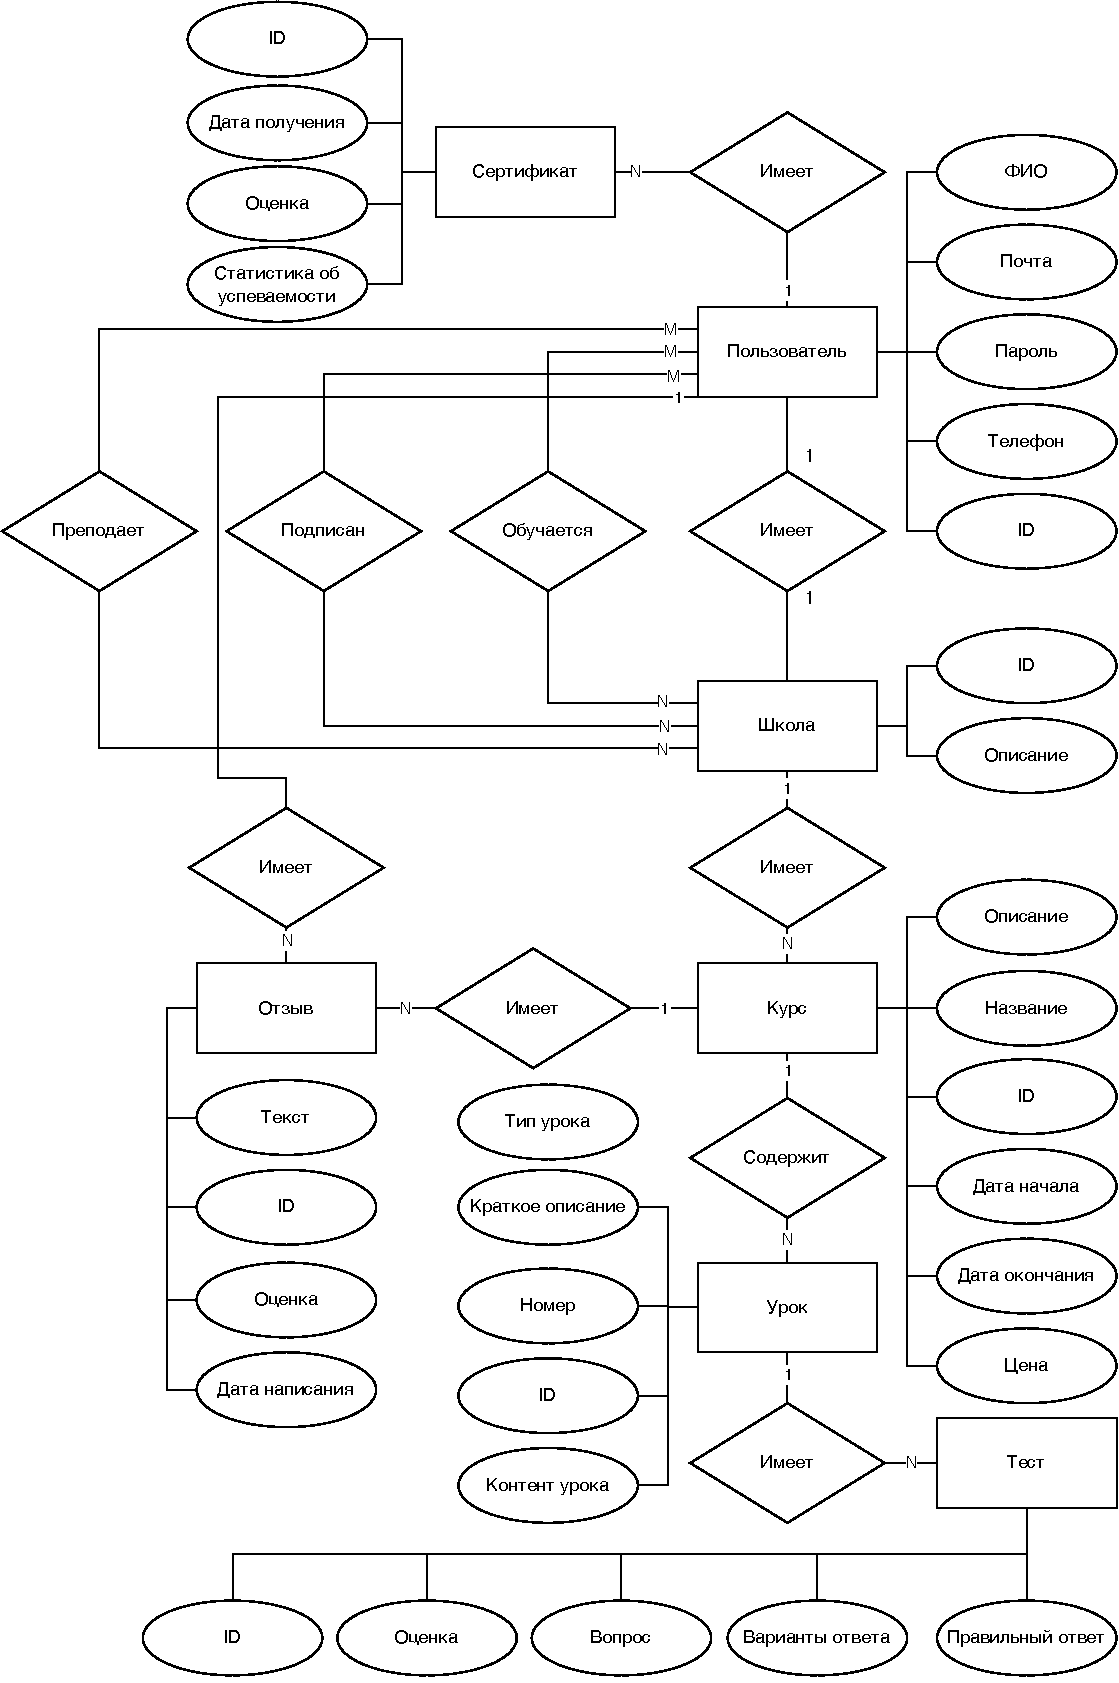
\includegraphics[height=0.9\textheight]{inc/img/er.pdf}
	\caption{ER-диаграмма сущностей в нотации Чена}
	\label{img:er}
\end{figure}

\section{Формализация ролей}
В данной работе выделяются следующие роли пользователей:
\begin{itemize}
    \item гость -- неавторизованный пользователь, который может посматривать информацию о курсе,
    авторизоваться, зарегистрироваться;
    \item пользователь -- авторизованный пользователь, может просматривать курсы, проходить, оплачивать их,
    по завершении курса получать сертификат и отчет об успеваемости и оставлять отзывы,
    стать преподавателем, создать собственную школу и курсы в ней,
    а также присоединиться к существующей школе в качестве преподавателя;
    \item администратор -- авторизованный пользователь, может создавать, изменять и удалять пользователей, курсы, школы, уроки, отзывы.
\end{itemize}

\section{Формализация задачи}
Необходимо спроектировать базу данных для хранения информации о студентах и преподавателях, школах, курсах и уроках, входящих в состав курса, а также об отзывах пользователей.
Разработанное приложение для доступа к базе данных должно предоставлять каждому пользователю возможность покупать и проходить курсы различной тематики. Также у каждого пользователя должна быть возможность создать собственную школу и образовательную программу
или присоединиться к уже существующей школе в качестве преподавателя или составителя курса.

По прохождении курса пользователь должен иметь возможность получить сертификат о завершении обучения,
включающий подробное описание его успеваемости и итоговую оценку. Диаграмма вариантов использования приведена на рисунке \ref{img:usecase}.

\begin{figure}[H]
	\centering
	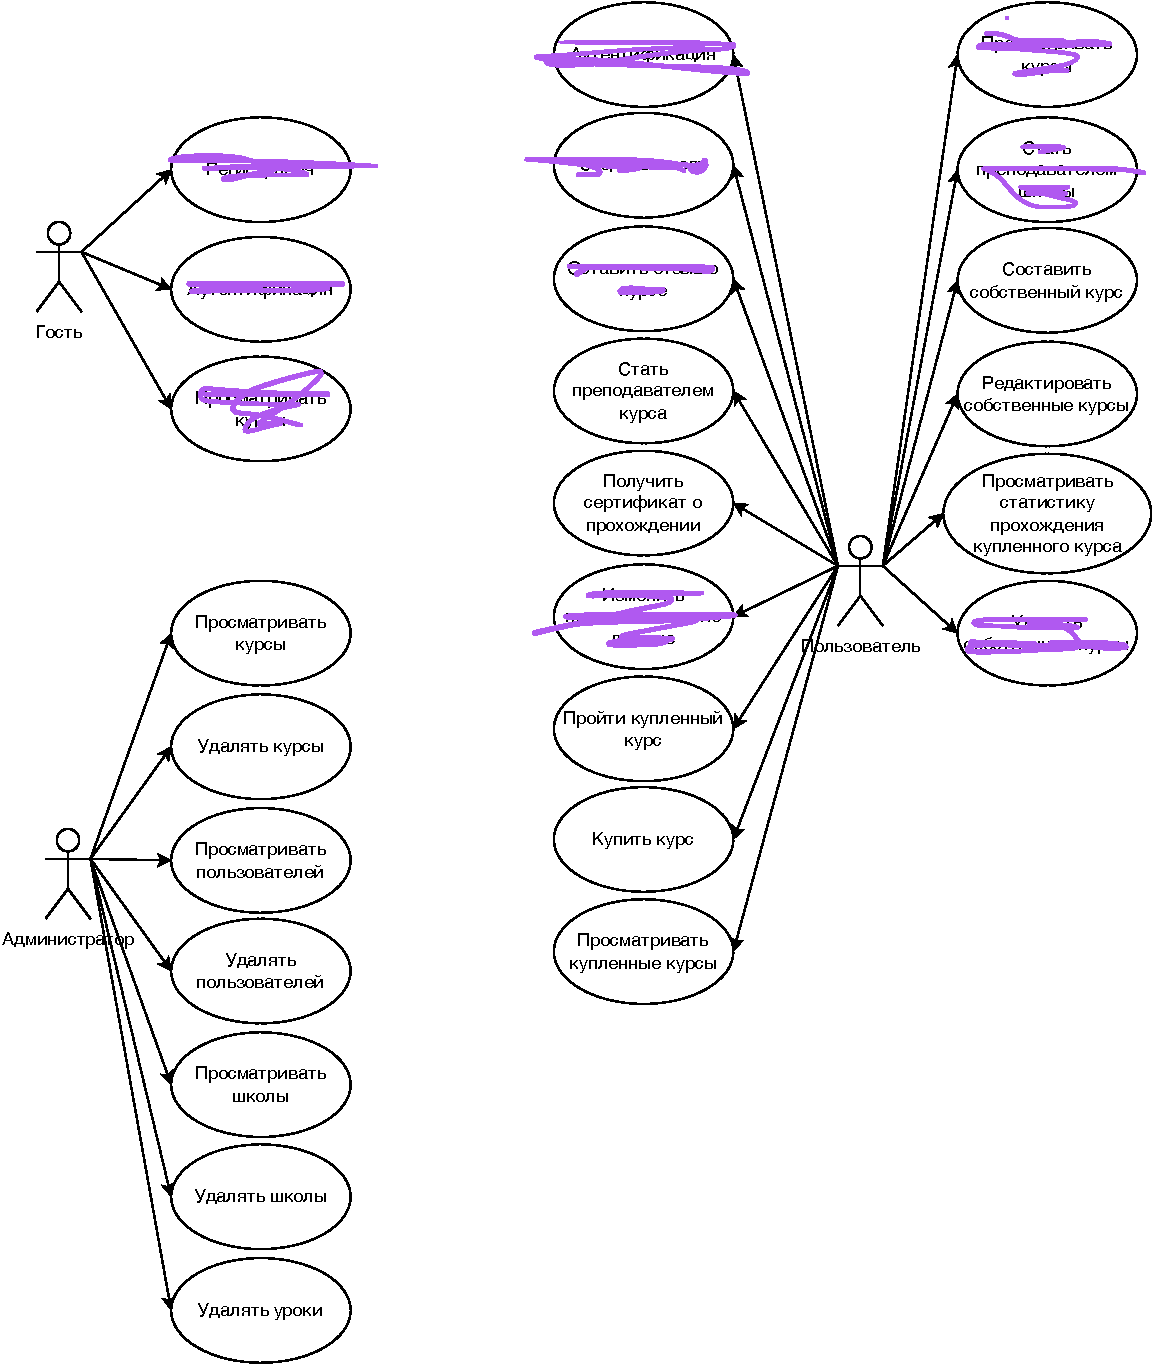
\includegraphics[height=0.7\textheight]{inc/img/usecase.pdf}
	\caption{Диаграмма вариантов использования}
	\label{img:usecase}
\end{figure}

\section{Анализ баз данных}
База данных -- совокупность данных, хранимых в соответствии со схемой данных, манипулирование которыми выполняют в соответствии с правилами средств моделирования данных.

СУБД -- совокупность языковых и программных средств общего или специального назначения, обеспечивающих управление созданием и использованием баз данных~\cite{williams}.

Модель данных представляет собой абстрактное, логическое описание элементов, таких как объекты и операции, которые в совокупности образуют виртуальную систему управления данными, с которой взаимодействует пользователь. Объекты модели описывают структуру данных, в то время как операции отражают их поведение.

Базы данных можно классифицировать по модели хранения на несколько типов:
\begin{itemize}
    \item дореляционные модели данных --- включают иерархические, сетевые модели и системы, использующие инвертированные списки.
    \item реляционные модели данных --- основываются на таблицах, что делает их более гибкими и простыми в использовании.
    \item нереляционные модели данных --- ориентированы на расширенные возможности работы с данными, выходящие за рамки реляционной парадигмы.
\end{itemize}

\subsection*{Дореляционные модели}
Дореляционные базы данных представляют собой тип баз данных, который не использует табличную модель данных. Вместо этого, они хранят данные в структурах, таких как деревья, графы или объекты. 

\subsection*{Реляционная модель данных}
Реляционные базы данных основаны на реляционной модели данных, где данные организованы в виде таблиц, которые имеют связи между собой. Каждая таблица представляет отдельную сущность, а связи между таблицами устанавливаются с помощью ключевых полей. Важным свойством реляционных баз данных является их способность удовлетворять требованиям ACID~\cite{acid}: атомарность, согласованность, изоляция, устойчивость. Примерами реляционных баз данных являются MySQL~\cite{mysql}, PostgreSQL~\cite{postgres}, Oracle~\cite{oracle} и SQL Server~\cite{sql-server}.

\subsection*{Нереляционная модель данных}
Постреляционные базы данных -- это базы данных, которые разработаны для обработки и анализа больших объемов данных. В отличие от реляционных баз данных, основанных на таблицах, нереляционные базы данных предлагают более гибкие способы хранения данных, что делает их подходящими для определенных типов задач, таких как обработка больших объемов данных, работа с распределенными системами и требование высокой производительности. Примерами постреляционных баз данных являются Apache Hadoop~\cite{hadoop}, Apache Cassandra~\cite{cassandra} и Apache Spark~\cite{spark}.

\section{Вывод из аналитической части}
С учетом задачи была выбрана реляционная модель хранения данных, так как предметная область может быть представлена в виде таблиц и должна удовлетворять требованиям ACID.
